\documentclass[12pt]{report}

% includes
\usepackage{geometry}           % page size
\usepackage[utf8]{inputenc}     % encoding
\usepackage{palatino}           % font
\usepackage[english]{babel}    % language
\usepackage{graphicx}           % images
\usepackage{float}
\usepackage{indentfirst}        % indentation
\usepackage[nottoc]{tocbibind}  % table of contents style
\usepackage[unicode]{hyperref}  % references from the table of contents
\usepackage[font=footnotesize,labelfont=bf]{caption}
\usepackage{amsmath}
\usepackage{amssymb}
\usepackage{amsthm}
\graphicspath{{./images/}}

% includes options
\geometry{  a4paper,            % scientific thesis standard
            left=3cm,
            right=2cm,
            top=2cm,
            bottom=2cm,
 }
\graphicspath{{images/}}        % path where the images are located
\setlength{\parindent}{1cm}     % paragraph indentation

% other options
\linespread{1.5}                % space between lines
\renewcommand*\contentsname{Cuprins}    % table of contents name

% the document content
\begin{document}
    % macros (global)
    \newcommand{\university}    {Universitatea "Alexandru-Ioan Cuza" din Iași}
\newcommand{\universityg}   {Universității "Alexandru-Ioan Cuza" din Iași} % genitive
\newcommand{\faculty}       {Facultatea de informatică}
\newcommand{\facultyg}      {Facultății de informatică} % genitive
\newcommand{\speciality}    {Studii Avansate în Informatică}
\newcommand{\promotion}     {2022}                                  %<---------

\newcommand{\thesistype}    {Lucrare de disertație}
\newcommand{\thesistitle}   {Methods for assessing clustering stability in single-cell expression datasets}    %<---------

\newcommand{\authorlast}    {Munteanu}                               %<---------
\newcommand{\authorfirst}   {Andi}
\newcommand{\authornamefl}  {\authorfirst \space \authorlast} % first name first
\newcommand{\authornamelf}  {\authorlast \space \authorfirst} % last name first
\newcommand{\authorbirth}   {01 ianuarie 2018}                      %<---------
\newcommand{\authoraddress} {România, jud. Iași, mun. Iași, calea Buzăului, nr. 25, bl. A, et. 5, ap. 45} %<---------
\newcommand{\authorcnp}     {1234567891234}                         %<---------

\newcommand{\session}       {Iulie, 2022}                       %<---------
\newcommand{\coordinator}   {Conf. Dr. Liviu Ciortuz}               %<---------

\newcommand{\dottedline}    {............................}
\renewcommand{\qedsymbol}{$\blacksquare$}
\renewcommand{\footnotesize}{\scriptsize} 
    
    % front-matter
    \pagenumbering{gobble}

    % define the cover page
\begin{titlepage}
    \begin{center}
        % the university and faculty
        \large
        \MakeUppercase{\university}
        
        \LARGE
        \textbf{\MakeUppercase{\faculty}}
        
        % the faculty logo
        \vspace{1cm}
        
\includegraphics[width=0.3\textwidth]{logoFii.png}
        
        % thesis title
        \vspace{1cm}
        \Large
        \MakeUppercase{\thesistype}
        
        \vspace{0.5cm}
        \LARGE
        \textbf{\thesistitle}
        
        % author
        \vspace{2cm}
        \Large
        propusă de
        
        \vspace{0.5cm}
        \LARGE
        \textbf{\authornamefl}
        
        % session
        \vfill
        \Large
        \textbf{Sesiunea:} \session
        
        % scientific coordinator
        \vspace{2cm}
        \Large
        Coordonator științific
        
        \vspace{0.5cm}
        \LARGE
        \textbf{\coordinator}
    \end{center}
\end{titlepage}
    % define the title page
\begin{titlepage}
    \begin{center}
        % the university and faculty
        \large
        \MakeUppercase{\university}
        
        \LARGE
        \textbf{\MakeUppercase{\faculty}}
        
        % thesis title
        \vspace{6cm}
        \huge
        \textbf{\thesistitle}
        
        % author
        \vspace{2cm}
        \LARGE
        \textbf{\authornamefl}
        
        % session
        \vfill
        \Large
        \textbf{Sesiunea:} \session
        
        % scientific coordinator
        \vspace{3cm}
        \Large
        Coordonator științific
        
        \vspace{0.5cm}
        \LARGE
        \textbf{\coordinator}
    \end{center}
\end{titlepage}
    \vspace*{\fill}

\begin{flushright}
    Avizat, \\
    Îndrumător lucrare de licență, \\
    \coordinator. \\
    Data: \dottedline \hspace{1cm} Semnătura: \dottedline
\end{flushright}

\vspace{1cm}
\begin{center}
    \large
    \textbf{Declarație privind originalitatea conținutului lucrării de licență}
\end{center}

Subsemnatul \textbf{\authornamelf} domiciliat în \textbf{\authoraddress}, născut la data de \textbf{\authorbirth}, identificat prin CNP \textbf{\authorcnp}, absolvent al \facultyg, \textbf{\faculty} specializarea \textbf{\speciality}, promoția \promotion, declar pe propria răspundere cunoscând consecințele falsului în declarații în sensul art. 326 din Noul Cod Penal și dispozițiile Legii Educației Naționale nr. 1/2011 art. 143 al. 4 și 5 referitoare la plagiat, că lucrarea de licență cu titlul \textbf{\thesistitle} elaborată sub îndrumarea domnului \textbf{\coordinator}, pe care urmează să o susțin în fața comisiei este originală, îmi aparține și îmi asum conținutul său în întregime.

De asemenea, declar că sunt de acord ca lucrarea mea de licență să fie verificată prin orice modalitate legală pentru confirmarea originalității, consimțind inclusiv la introducerea conținutului ei într-o bază de date în acest scop.

Am luat la cunoștință despre faptul că este interzisă comercializarea de lucrări științifice în vederea facilitării falsificării de către cumpărător a calității de autor al unei lucrări de licență, de diplomă sau de disertație și în acest sens, declar pe proprie răspundere că lucrarea de față nu a fost copiată ci reprezintă rodul cercetării pe care am întreprins-o.

\begin{flushright}
    Data: \dottedline \hspace{6cm} Semnătura: \dottedline
\end{flushright}

\vspace*{\fill}
\pagebreak
    \vspace*{\fill}
\begin{center}
    \large
    \textbf{Declarație de consimțământ}
\end{center}

Prin prezenta declar că sunt de acord ca lucrarea de licență cu titlul \textbf{\thesistitle}, codul sursă al programelor și celelalte conținuturi (grafice, multimedia, date de test, etc.) care însoțesc această lucrare să fie utilizate în cadrul \facultyg.

De asemenea, sunt de acord ca \faculty \space de la \university, să utilizeze, modifice, reproducă și să distribuie în scopuri necomerciale programele-calculator, format executabil și sursă, realizate de mine în cadrul prezentei lucrări de licență.

\begin{flushright}
    Absolvent \textbf{\authornamefl} \\
    \vspace{0.5cm}
    Data: \dottedline \hspace{6cm} Semnătura: \dottedline
\end{flushright}
\vspace*{\fill}
\pagebreak
    % table of contents
    \tableofcontents

    % chapters
    \setcounter{page}{1}
    \pagenumbering{arabic}
    
    \chapter*{Acknowledgments} 
\addcontentsline{toc}{chapter}{Acknowledgments}

I acknowledge the support and supervision of Professor Liviu Ciortuz. I am indebted for the patience and knowledge shared with me over the past few years. During my MSc, I was also fortunate to collaborate closely with the Core Bioinformatics group at the Cambridge Stem Cell Institute and get acquainted with cutting-edge problems in bioinformatics. 

This thesis is based on the ClustAssess manuscript \cite{clustassess} to which I contributed as co-author. All the figures used in the last three chapters are also presented in the paper. The writing of the article and the development of the \verb|ClustAssess| package was done under the supervision and mentorship of professor Irina Mohorianu and Arash Shahsavari (Core Bioinformatics Group, Cambridge Stem Cell institute), as part of my internship at the Cambridge Stem Cell Institute during the summer of 2021. The experiments and benchmarks were performed on the CSCI computing infrastructure. The ClustAssess code is publicly available on the Core Bioinformatics GitHub repository \url{https://github.com/Core-Bioinformatics/ClustAssess} and can be used for academic purposes under the MIT license.
    \chapter*{Introduction} 
\addcontentsline{toc}{chapter}{Introduction}

The unsupervised clustering of points remains an essential tasks in data processing and machine learning. Its relevance is underlined by the diversity of domains where clustering plays an important role. One of these relates to the bioinformatics field, where the clustering became essential in the identification process of cell types \cite{Kiselev2019a} in single-cell RNA-seq datasets or the inference of cell trajectories \cite{Saelens2019}.

As the size of the dataset grew to the size of millions of cells \cite{Svensson2020a}, these tasks have become less obvious: the cell annotations has become more reliant on the output of the clustering algorithms. The challenge was then to improve the accuracy of the classification methods as well as their performance and scalability.

One of the earliest clustering techniques is k-means \cite{Lloyd1982}, which gained popularity due to its simplicity and intuitive approach. Its bias on the size and shape of the clusters determined the introduction of other types of clustering such as density-based (DBSCAN \cite{ester1996}), hierarchical, distribution-based (EM \cite{Dempster1977}).

In the last decades the storage of data in graph-based structures has become more relevant \cite{cook2006mining}, as it was able to capture the relationship between observations. Single-cell analysis is one of the domains where graphs are the natural structure to represent the data, as it can keep the information about the relationship between cells. This lead to the introduction of a new type of clustering methods, namely the graph clustering.

While there are many approaches that were proposed to solve this problem, one of the methods that has become to be adopted at a larger scale was the community detection. This state-of-the art of this category of methods is represented by the Louvain \cite{Blondel2008b} algorithm, which takes a two-step approach to perform a greedy optimisation of an objective (also called quality in literature) function that attempts to define a good graph partitioning. The algorithm was furtherly optimised and improved in later variants such as Louvain with multi-level refinement \cite{Rotta2011}, Smart Local Moving \cite{Waltman2013} and Leiden \cite{Traag2019a}.

The limitation that single-cell analysis faced was that its default data representation structure was not a graph, but a matrix that describe the expression levels of the present cells. To address this issue, the PhenoGraph \cite{Levine2015} was introduced and proposed a pipeline of clustering the data in three steps: dimensionality reduction using approximate PCA (for example, the Lanczos bidiagonalization method \cite{Baglama2016IRLBAFP}) or UMAP \cite{mcinnes2018uniform}, graph construction using kNN \cite{Xu2015}, and graph clustering using community detection.

This pipeline was incorporated and implemented in different frameworks used specifically for processing the single-cell data, like Seurat \cite{Hao2021}, Monocle \cite{Cao2019} or SCANPY \cite{Wolf2018}. In this thesis we will compare how the PhenoGraph pipeline was included in the Seurat and Monocle packages and will analyze the main technical sources that lead to divergent results between them.

This analysis raised the question of the pipeline stability when the random seed changes, as most of the algorithms involved contain at least one stochastic component. The instability cause by random seed was issued in previous works. Some of the approaches were to modify the algorithm as in kmeans++ \cite{kmeanspp} or to add noise to data as in the clust-perturb algorithm \cite{STACEY2021}. We propose \verb|ClustAssess|, a R package that provides a pipeline meant to visually guide the user into choosing a configuration of parameters that leads to results where the seed effect is negligible, without performing any changes to the methods or the original data.

The stability is inferred by running the pipeline multiple times with different seeds and compare the results using the Element-Centric Similarity score \cite{Gates2019}. This score is a clustering comparing tool that does not have any bias regarding the size of the clusters, their shape or the problem of matching, like the traditional measurements (such as NMI \cite{McDaid2015} or ARI \cite{Collins1988}). Our package also provides an optimized implementation of the ECS score that scales well on larger datasets.


    
    \chapter{Description of methods}

This chapter contains informations about the methods used for graph clustering, the sequencing and processing the biological data and eventualy mentions of other works / papers that were focusing on assessing the robustness on changing the seed.

\section{Graph Clustering}

\subsection{Short intro about what graph clustering is}

\subsection{Why graph clustering instead other traditional methods such as k-means, density based techniques etc}

\subsection{Types of graph clustering}

\subsection{Community detection - Optimizing the quality function}

\subsection{Louvain}

\subsection{Louvain refined}
\subsection{SLM}
\subsection{Leiden}
\subsection{}

\section{Element-Centric Similarity}

Pellentesque pulvinar pellentesque habitant morbi tristique senectus et. Ornare suspendisse sed nisi lacus sed viverra tellus in hac. Non sodales neque sodales ut etiam sit. In hendrerit gravida rutrum quisque non. Diam quam nulla porttitor massa id neque aliquam. Diam sit amet nisl suscipit adipiscing bibendum est ultricies integer. Cras fermentum odio eu feugiat pretium nibh ipsum. Egestas integer eget aliquet nibh praesent tristique magna. Porttitor eget dolor morbi non arcu risus quis varius quam. Gravida rutrum quisque non tellus orci. Diam volutpat commodo sed egestas egestas.

\section{Intro info about biological data and sequencing techniques}
    \chapter{The importance of parameter values in the clustering output}

\section{Monocle and Seurat}
As stated in the previous chapter, the PhenoGraph pipeline was widely adopted in the task of processing biological data, due to its efficiency and quality of results. The pipeline was incorporated and implemented in various programming languages.

The most frequently used R packages that perform single-cell data processing are Seurat (currently on the third version) \cite{Hao2021} and Monocle (currently at the third version) \cite{Cao2019}. Both packages use the PhenoGraph method for the cell clustering. The goal of this chapter is to evaluate the output of the two packages and compare the results side by side.

\section{Data used for experiments}
To perform this comparison, we used the Cuomo data \cite{Cuomo2020}, an in-vitro SMART-seq dataset of human endoderm differentiation. The dataset contains 1880 cells extracted from six donors (hayt, naah, vils, pahc, melw and qunz) at four different timepoints. The cells are in expressed in approximately 30 000 genes. The dataset was preprocessed by removing the cells that are expressed in less than 200 features and the genes that are expressed in less than three cells. MT (mitochondrial) and RP (ribosomal protein) genes were also excluded from the feature set.

The purpose of this thesis is to analyze the clustering pipeline, therefore the preprocessing parameters (normalization and scaling) are done in the same manner for both packages.

\section{Algorithms used in the pipeline}
In chapter one we presented the steps that are involved in the PhenoGraph pipeline, namely the dimensionality reduction, the graph construction and the community detection. Each step can be performed by a varying number of algorithms. Therefore, in order to compare the two R packages, we must identify the algorithms that they are using in the clustering pipeline (see Table \ref{tab:s4-m3-methods}).

For the dimensionality reduction, both packages allow the usage of either linear methods (PCA) or non-linear ones (UMAP and tSNE). The developers of the both packages recommend performing the PCA reduction on the raw data, followed by tSNE or UMAP. The graph construction is performed using the kNN based method. For the community detection, Monocle uses the Louvain and Leiden alogrithms, whereas Seurat can cluster the cells using Louvain with multi-level refinement and SLM, too.

We note that all the algorithms involved in the clustering pipeline contain at least one stochastic component, therefore 

\begin{table}[]
    \begin{tabular}{|l|l|l|l|}
        \hline
                         & \textbf{Dim reduction}    & \textbf{Graph construction} & \textbf{Graph clustering} \\ \hline
        \textbf{Seurat}  & \begin{tabular}[c]{@{}l@{}}PCA followed\\ by tSNE or UMAP\end{tabular} & \begin{tabular}[c]{@{}l@{}}kNN based\\ support for SNN\end{tabular}   & \begin{tabular}[c]{@{}l@{}}Louvain, Louvain refined,\\ SLM, Leiden\end{tabular} \\ \hline
        \textbf{Monocle} & \begin{tabular}[c]{@{}l@{}}PCA followed\\ by tSNE or UMAP\end{tabular} & \begin{tabular}[c]{@{}l@{}}kNN based\\ support for SNN\end{tabular}   & Louvain, Leiden           \\ \hline
    \end{tabular}
    \caption{\label{tab:s4-m3-methods}The algorithms used by Monocle and Seurat inside the Phenograph pipeline}
\end{table}

\section{Comparing the results}

\begin{figure}[H]
    \centering
    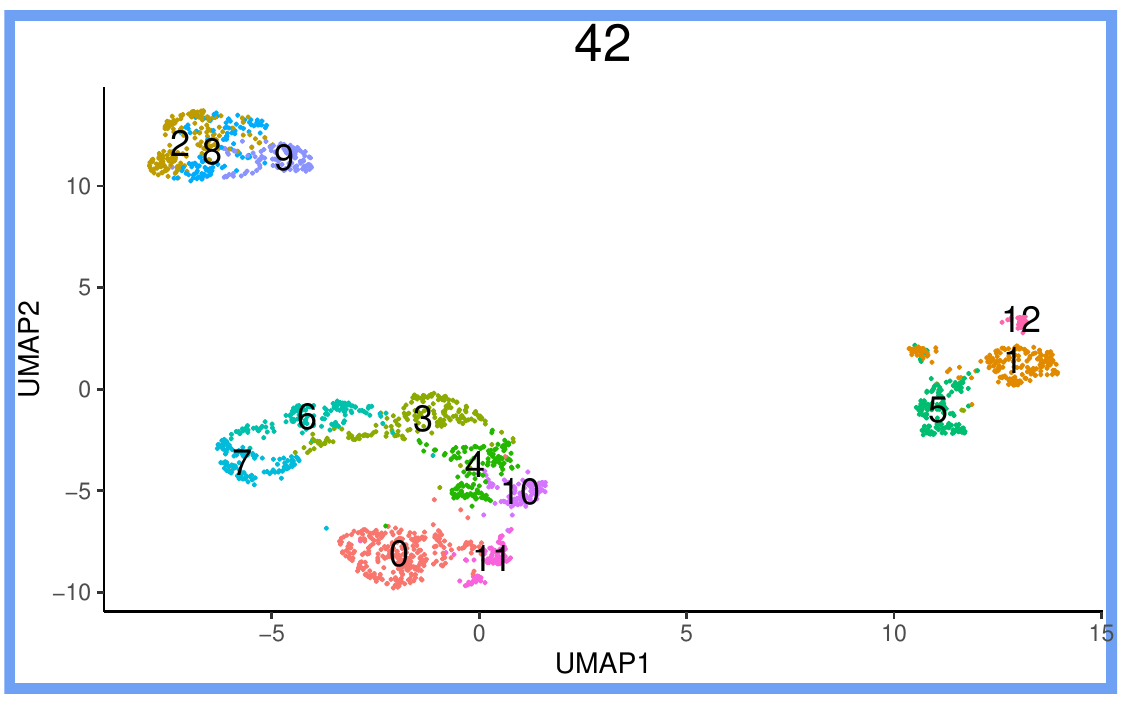
\includegraphics[width=7cm]{2_S1.png}
    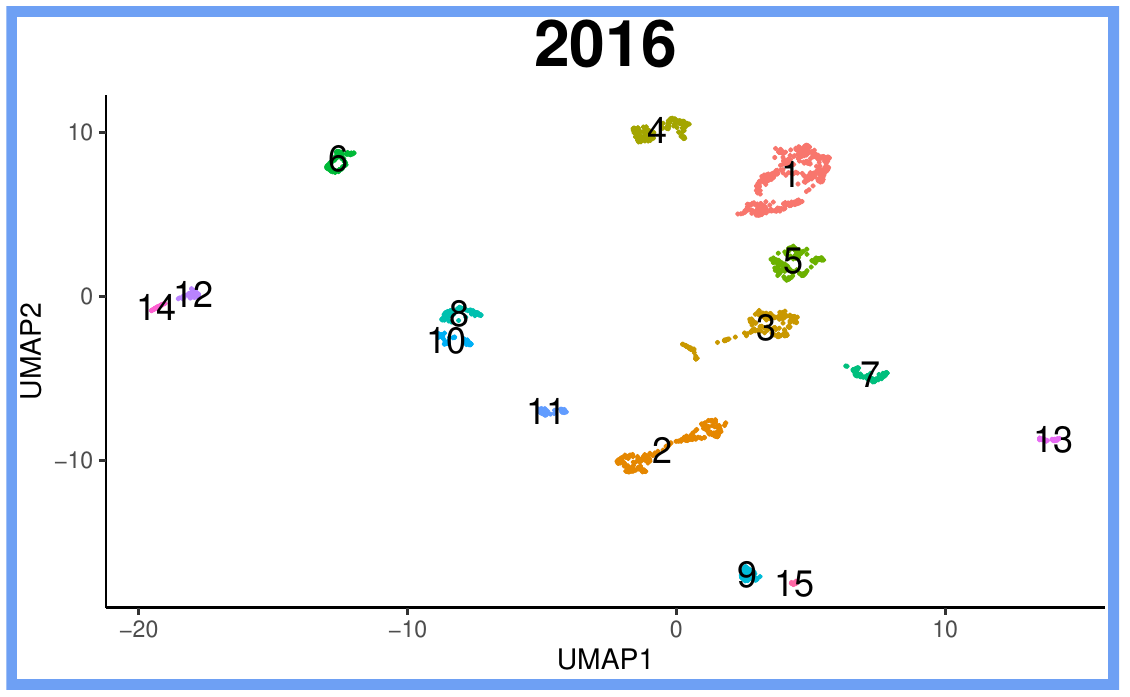
\includegraphics[width=7cm]{2_M1.png}
    \caption{\label{fig:s4-m3-default}Clustering distribution with default parameters for Monocle (right) and Seurat (left). The title indicates the default random seed that is used.}
\end{figure}

If the Cuomo \cite{Cuomo2020} dataset is clustered using the Monocle and Seurat packages with default parameters, significantly different outputs are produced, as it can be observed in Figure \ref{fig:s4-m3-default}. Firstly, there are differences with respect to the dimensionality reduction. The cells are scattered in multiple islands in the Monocle package, whereas Seurat obtains a more compact grouping. Also, the two packages disagree regarding the number of clusters: Seurat outputs 13 clusters, Monocle 15.

The biological interpretation of the data heavily relies on the clusters' structure. Thus, is expected for the discrepancies between the two packages to extend over the marker identification and the biological interpretation. The question we pose is whether the divergence between Monocle and Seurat has technical (such as the implementation of the clustering pipeline) or biological (such as additional pre- or post-processing steps that rely on the sequencing information) causes.

\section{Aligning the results}
We started by analyzing the tehnical differences between the two packages. This involves implementation discrepancies, but also different values of the parameters involved in the clustering process. Our analysis will follow the PhenoGraph pipeline and we will compare the two packages regarding the three steps.

\subsection{Dimensionality reduction}
As stated in the previous sections, both Seurat and Monocle suggest applying PCA on the raw dataset and UMAP or tSNE afterwards. The default choice for non-linear dimensionality reduction is UMAP. As for the implementation, both packages are using the same R packages: \verb|irlba| for PCA (citation) and \verb|uwot| for UMAP (citaton).

\subsubsection{PCA}
The output of the PCA can be affected by parameters such as the number of principal components or the precision of the calculation (the \verb|irlba| package performs an approximate PCA calculation), but the difference between the packages lies in the feature space. Although the data contains up to 30 000 genes, most of them are not appropiate for describing the cells behaviour, as they would introduce more noise than perform any significant separation. Thus, the standard in the processing of the biological data is to choose a relatively small subset of genes that contain discriminative information. By default, Monocle uses all genes, but Seurat performs the PCA only on the genes that have the most variability (citation) (also reffered in literature as highly variable - or HV - genes). Figure \ref{fig:s4-m3-pca} illustrates how the feature set affects the topology. If Seurat uses all genes for PCA, the resulting embedding will contain numerous small islands (see panels S3 and S4). Using only HV genes in Monocle leads to more compact group of cells (see panels M3 and M4).

\subsubsection{UMAP}
The UMAP algorithm is signifcantly affected by three parameters:
\begin{itemize}
    \item \textit{the distance metric} that is used in the original space
    \item \textit{the number of neighbours} that is used for building the graph
    \item \textit{the minimum distance} which determines how separated should points be in the low dimensional space. Low values lead to dense groups, while higher values are more preferable for visualisation.
\end{itemize}

Monocle and Seurat agree on the cosine measurement as the distance metric, but the other two parameters have different values in these packages: the minimum distance is 0.3 in Seurat and 0.1 in Monocle, and the number of neighbours is 30 in Seurat and 15 in Monocle. Figures \ref{fig:s4-m3-min-dist} and \ref{fig:s4-m3-n-neigh-umap} highlight the effect of these parameters on the toplogy of the data. Aligning their values for the two packages leads to identical low dimensional representation of the cells, as it can be seen in panels S7 and M8 of the figure \ref{fig:s4-m3-n-neigh-umap}.

\begin{figure}[H]
    \centering
    \makebox[\textwidth][c]{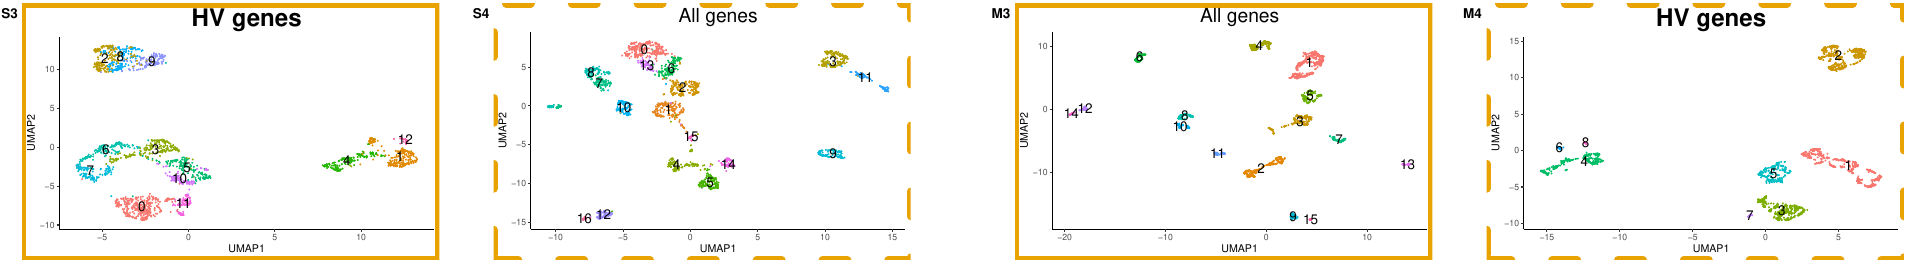
\includegraphics[width=1.2\linewidth]{2_pca_genes.png}}
    \caption{\label{fig:s4-m3-pca}Clustering distribution with default parameters for Monocle (left) and Seurat (right). The title indicates the default random seed that is used.}
\end{figure}


\begin{figure}[H]
    \centering
    \makebox[\textwidth][c]{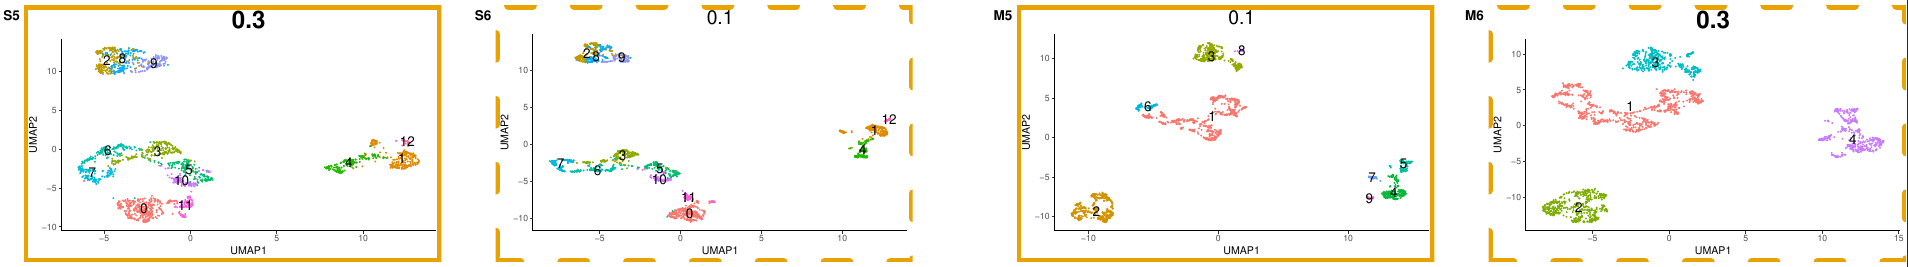
\includegraphics[width=1.2\linewidth]{2_umap_min_dist.png}}
    \caption{\label{fig:s4-m3-min-dist}Clustering distribution with default parameters for Monocle (left) and Seurat (right). The title indicates the default random seed that is used.}
\end{figure}

\begin{figure}[H]
    \centering
    \makebox[\textwidth][c]{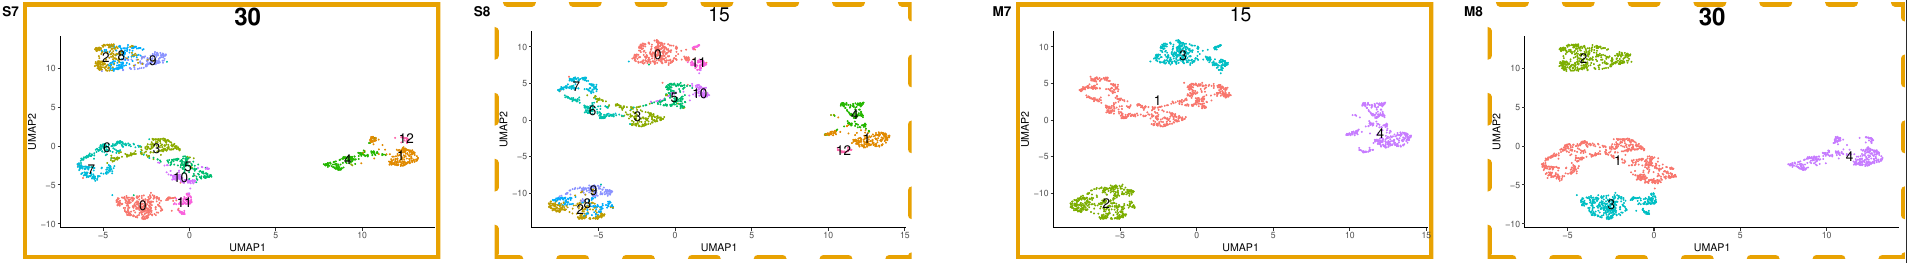
\includegraphics[width=1.2\linewidth]{2_umap_n_neigh.png}}
    \caption{\label{fig:s4-m3-n-neigh-umap}Clustering distribution with default parameters for Monocle (left) and Seurat (right). The title indicates the default random seed that is used.}
\end{figure}

\subsection{Graph construction}
Both packages use the kNN-based method of building the graph based on the reduced space. The calculation of the nearest neighbours is done by the method implemented in the \verb|RANN| package (citation). The output is affected by the embedding that is used as a base for the graph construction, the number of neighbours (or simply \textit{k}) and the graph type.

Both Monocle and Seurat agree upon the value of 20 nearest neighbours. As for the base embedding, Seurat builds the graph on the reduced space obtained by PCA, while Monocle uses the low dimensional data from UMAP. As Figure \ref{fig:s4-m3-graph-base} suggests, changing the base embedding can affect the clustering output. On the Cuomo data, the number of clusters is lower when PCA is used as base embedding compared to UMAP for both packages (this can be observed by comparing panels S9 with S10 an M9 with M10 respectively).

When it comes to calculating the Shared Nearest Neighbour graph, the two packages have their own implementation. Although they are synonymous in the most of the cases, there are some differences that impact the final structure of the resulting graph.

\subsubsection{Self-neighbours}
The major discrepancy between them relates to the usage of the self-neighbours. A \textit{self-neighbour} refers to label a point as a near neighbour of itself. Seurat uses self-neighbours, while Monocle doesn't.

The importance of self-neighbours is illustrated on Figure \ref{fig:s4-m3-snn-1}. Setting $k = 5$, we calculate the neighbourhoods for the fourth and the fifth points. If we include the self-neighbour, we get:

\[ \begin{aligned}
    N_5(4) = \{4,5,3,1,2\}& \\
    N_5(5) = \{5,4,3,2,1\}
    \end{aligned}
\]

Given that the SNN graph is calculated using the Jaccard Similarity Index of the neighbourhoods, the weight of the edge between these two nodes will be:

\[ W_{4,5} = \textrm{JSI}(N_5(4), N_5(5)) = \frac{|N_5(4) \cap N_5(5)|}{|N_5(4) \cup N_5(5)|} = \frac{5}{5} = 1 ,\]

which indicates a perfect similarity between the two points. However, not including the self-neighbours leads to the following results:

\[ \begin{aligned}
    N_5(4) = \{5,3,1,2,6\}& \\
    N_5(5) = \{4,3,2,1,7\}
    \end{aligned}
\]

The intersection between these neighbourhoods contains only three points, and the union contains seven. Thus, the weight assigned in this case would be $3 / 7 = 0.43$. Even if we decrease the value of $k$ from 5 to 4, the JSI would be $3 / 5 = 0.6$, which still does not reflect or indicate the reality of a perfect similarity between the two nodes.

Another discrepancy is presented in the example provided in the Figure \ref{fig:s4-m3-snn-2}. Using the same value for $k$, we calculate the neighbourhoods for the first and the sixth point. If we include the self-neighbour, we get:

\[ \begin{aligned}
    N_5(1) &= \{1,2,3,4,6\} \\
    N_5(6) &= \{6,7,8,9,1\}
    \end{aligned}
\]

The neighbourhoods sets of these two points point out that they are direct neighbours. Therefore, the weight of the edge between them is expected to be non-zero: $\displaystyle \frac{|N_6(4)  \cap N_6(6)|}{|N_6(4)  \cup N_6(6)|} = \frac{2}{8} = 0.25$. Excluding the self-neighbours leads to disjoint neighbourhoods:

\[ \begin{aligned}
    N_5(1) &= \{2,3,4,6,5\} \\
    N_5(6) &= \{7,8,9,1,10\}
    \end{aligned}
\]

Thus, not using the self-neighbours leads to the false conclusion that there is no similarity between direct neighbours.

\subsubsection{Indirect neighbours}
Another implementation difference between Seurat and Monocle relates to the indirect neighbour. We consider two points to be \textit{indirect neighbours} if the intersection of their neighbourhoods is not disjoint. Looking at the third and eighth points from the example from Figure \ref{fig:s4-m3-snn-1} when $k = 6$, the intersection between their neighbourhoods is not empty ($\{5, 7\}$ for Seurat and $\{5,7,4,6\}$ for Monocle).

Even if the intersection is not empty, Monocle discards any use of the indirect neighbours. Thus, there will be an edge between two nodes only if they are direct neighbours.

\subsubsection{Scaling the weights}
Following the conclusion of the previous two differences, we can state that Monocle cannot build a graph that has an edge with weight 1.

\begin{proof} From the first difference, Monocle does not include the self-neighbours, therefore points that are direct neighbours will always have the JSI less than one, as the intersection will not include the points themselves. The only way to reach a perfect similarity is to have two points that are not direct neighbours, but share the same neighbourhood.

However, from the second difference, we know that in Monocle indirect neighbours are not taken into consideration. Therefore, even if we would obtain an edge with a weight of one between the two points, it will be discarded, given the restriction.
\end{proof}

The developers of the Monocle package decided to solve this limitation by performing a scaling of the weights to the interval $[0, 1]$. The issue of this approach is that it can affect the clustering output and the downstream partitioning result, as some quality function are scale variant (citation).

\subsubsection{Case study}
To prove the importance of these differences between the two implementations, we used the Cuomo \cite{Cuomo2020} dataset. The number of nearest neighbours is set to $k = 150$. Figure \ref{fig:s4-m3-snn-3} illustrates the difference between Monocle and Seurat results, shown for the neighbours of a point chosen from the datset.

The first two panels present the weight distribution of the edges incident to the chosen point when using Seurat (A) and Monocle (B). The third panel contains the absolute difference of the weights of the edges incident to direct neighbours. As it can be observed, the maximum difference is not greater than 0.012, which suggests that the two implementations behave similarly for direct neighbours when $k$ is reasonably high. Panel D shows the distribution of the weights incident to the indirect neighbours. The colour scale indicates that there is a reasonable amount of points where the weight has a value that may have an impact in the overall structure of the final graph.

\subsubsection{Aligning the SNN implementations}
After the analysis of the two implementations of the algorithm of building the SNN graph, we concluded that Seurat's is a more suitable choice. 

However, continuing the alignment process between the two packages, the graph type parameters is different. Seurat is building the SNN (the weighted) graph, while Monocle builds the unweighted one. The impact of this parameter is presented in the Figure \ref{fig:s4-m3-n-graph-type}, which suggests that using a weighted version of the same graph is influencing the clustering output.

\begin{figure}[H]
    \centering
    \makebox[\textwidth][c]{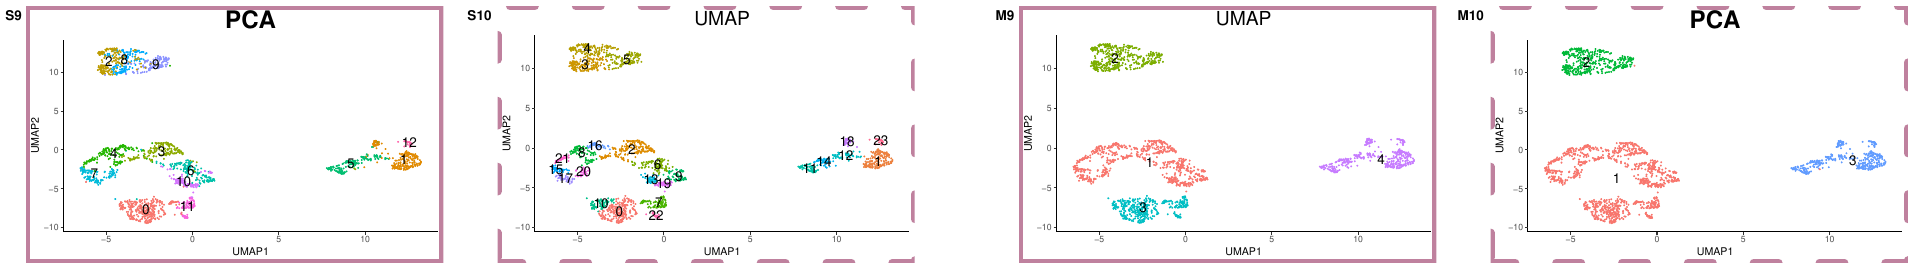
\includegraphics[width=1.2\linewidth]{2_graph_base.png}}
    \caption{\label{fig:s4-m3-graph-base}Clustering distribution with default parameters for Monocle (left) and Seurat (right). The title indicates the default random seed that is used.}
\end{figure}

\begin{figure}[H]
    \centering
    \makebox[\textwidth][c]{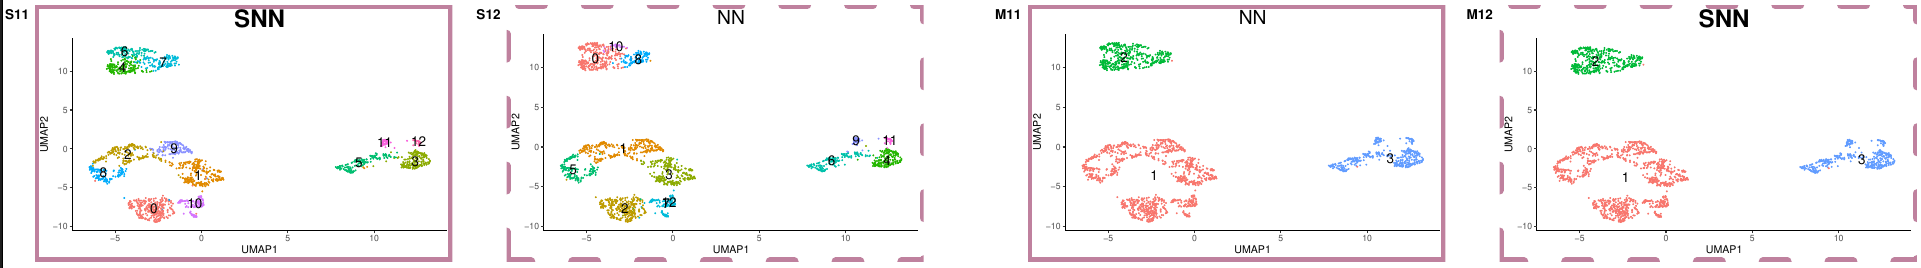
\includegraphics[width=1.2\linewidth]{2_graph_type.png}}
    \caption{\label{fig:s4-m3-n-graph-type}Clustering distribution with default parameters for Monocle (left) and Seurat (right). The title indicates the default random seed that is used.}
\end{figure}

\begin{figure}[H]
    \centering
    \makebox[\textwidth][c]{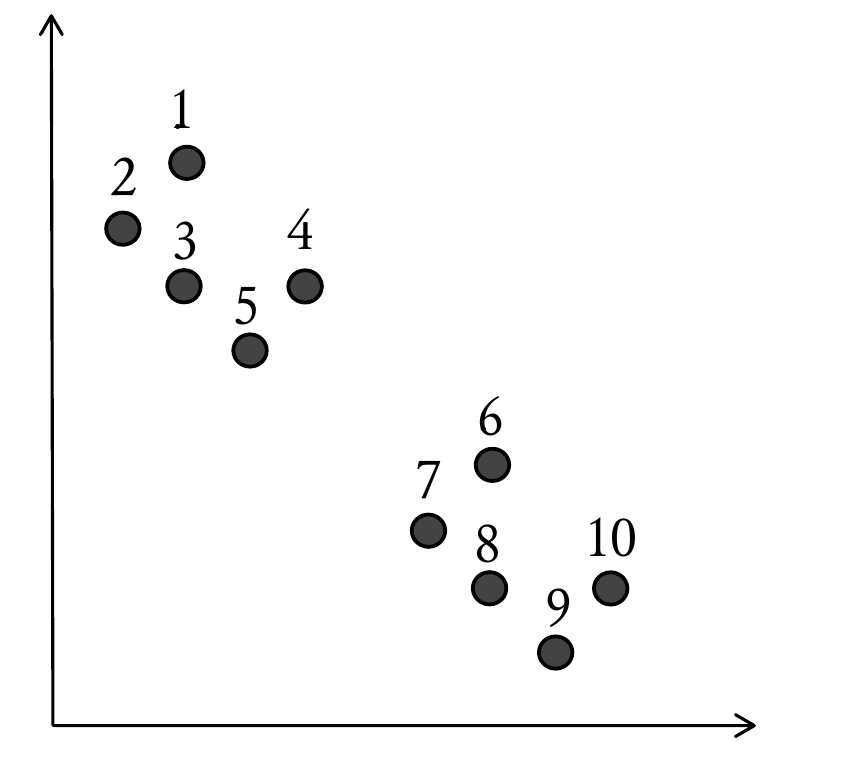
\includegraphics[width=5cm]{2_snn_issue_1.png}}
    \caption{\label{fig:s4-m3-snn-1}Clustering distribution with default parameters for Monocle (left) and Seurat (right). The title indicates the default random seed that is used.}
\end{figure}

\begin{figure}[H]
    \centering
    \makebox[\textwidth][c]{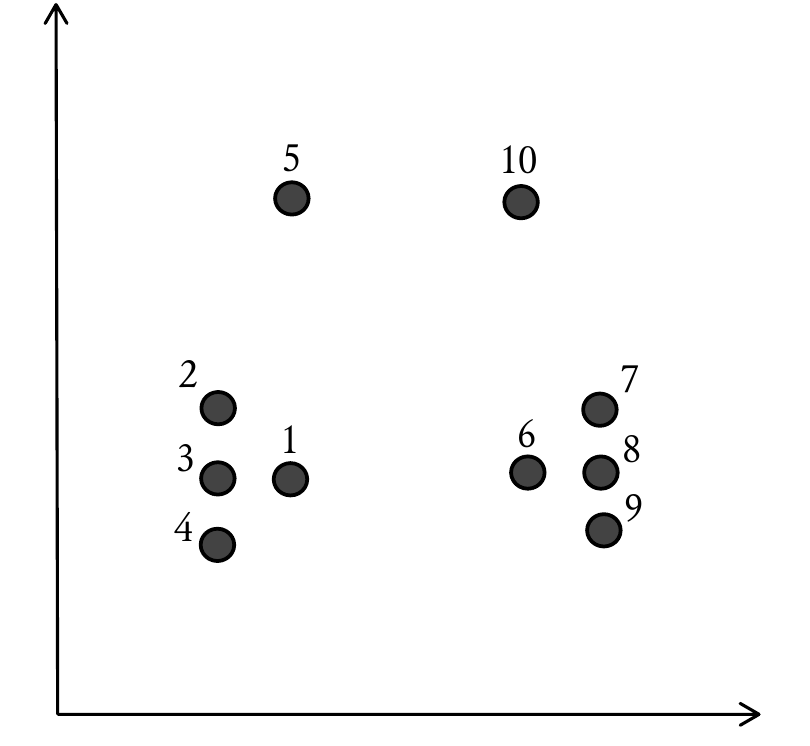
\includegraphics[width=5cm]{2_snn_issue_2.png}}
    \caption{\label{fig:s4-m3-snn-2}Clustering distribution with default parameters for Monocle (left) and Seurat (right). The title indicates the default random seed that is used.}
\end{figure}

\begin{figure}[H]
    \centering
    \makebox[\textwidth][c]{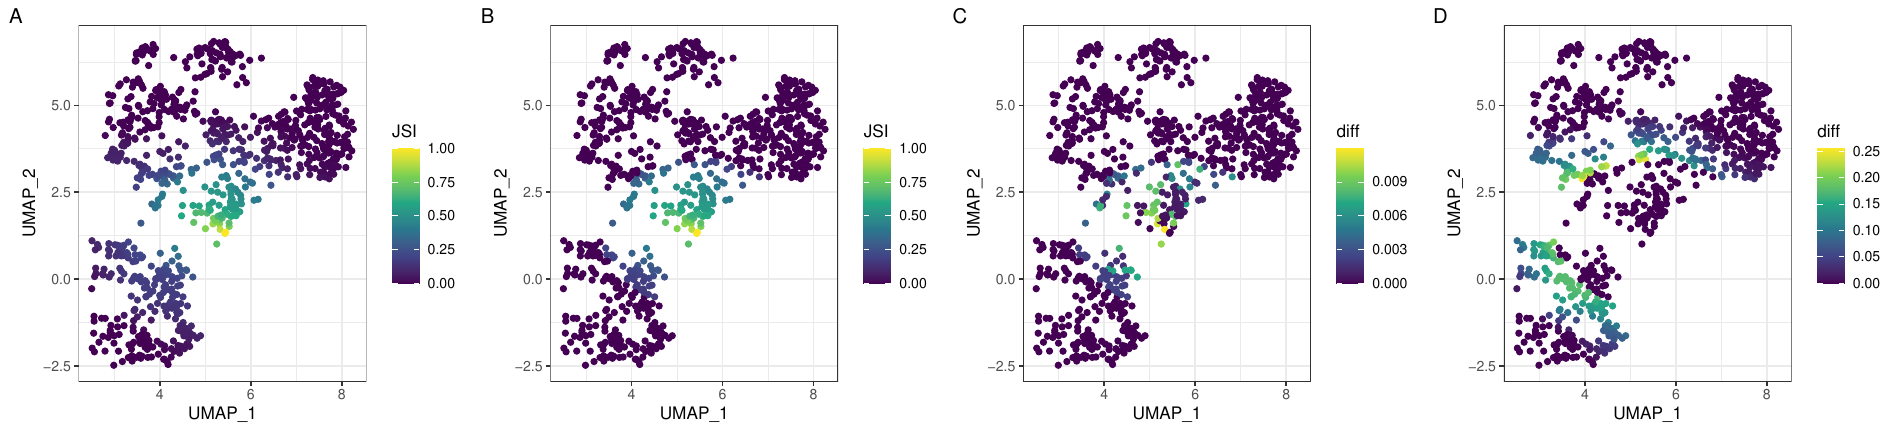
\includegraphics[width=1.2\textwidth]{2_snn_issue_3.png}}
    \caption{\label{fig:s4-m3-snn-3}Clustering distribution with default parameters for Monocle (left) and Seurat (right). The title indicates the default random seed that is used.}
\end{figure}
\subsection{Graph clustering}











    \chapter{ClustAssess}

Amet venenatis urna cursus eget. Quam vulputate dignissim suspendisse in est ante. Proin nibh nisl condimentum id. Egestas maecenas pharetra convallis posuere morbi. Risus viverra adipiscing at in. Vulputate eu scelerisque felis imperdiet. Cras adipiscing enim eu turpis egestas pretium aenean pharetra. In aliquam sem fringilla ut morbi tincidunt augue. Montes nascetur ridiculus mus mauris. Viverra accumsan in nisl nisi scelerisque eu ultrices vitae. In nibh mauris cursus mattis molestie a iaculis. Interdum consectetur libero id faucibus nisl tincidunt eget. Gravida in fermentum et sollicitudin ac orci. Suscipit adipiscing bibendum est ultricies. Etiam non quam lacus suspendisse. Leo urna molestie at elementum eu facilisis sed odio morbi. Egestas congue quisque egestas diam in arcu cursus. Amet consectetur adipiscing elit ut aliquam purus.

\section{Titlul secțiunii 1}

Eros donec ac odio tempor. Facilisi morbi tempus iaculis urna id volutpat. Faucibus in ornare quam viverra orci sagittis eu. Amet tellus cras adipiscing enim eu turpis egestas. Integer feugiat scelerisque varius morbi. Platea dictumst vestibulum rhoncus est pellentesque elit ullamcorper dignissim. Bibendum arcu vitae elementum curabitur. Eu nisl nunc mi ipsum faucibus. Id aliquet lectus proin nibh nisl condimentum id venenatis a. Cras adipiscing enim eu turpis egestas pretium. Quisque non tellus orci ac auctor augue mauris augue. Malesuada pellentesque elit eget gravida cum. Ut lectus arcu bibendum at. Massa id neque aliquam vestibulum morbi blandit. Posuere ac ut consequat semper viverra nam. Viverra adipiscing at in tellus integer feugiat scelerisque varius morbi. Morbi enim nunc faucibus a pellentesque sit amet porttitor eget. Eu feugiat pretium nibh ipsum consequat nisl vel. Nisl purus in mollis nunc sed.

\section{Titlul secțiunii 2}

Elementum sagittis vitae et leo duis ut diam quam nulla. Purus sit amet volutpat consequat mauris nunc. Tincidunt augue interdum velit euismod in pellentesque massa. Nunc sed augue lacus viverra vitae congue. Porttitor leo a diam sollicitudin. Faucibus pulvinar elementum integer enim. Adipiscing bibendum est ultricies integer quis auctor elit. Blandit aliquam etiam erat velit scelerisque in. A iaculis at erat pellentesque adipiscing commodo elit at. Erat nam at lectus urna duis. Consequat ac felis donec et. Fermentum posuere urna nec tincidunt praesent semper feugiat nibh sed. Proin gravida hendrerit lectus a. Pretium viverra suspendisse potenti nullam ac tortor vitae purus. Arcu cursus euismod quis viverra nibh cras pulvinar mattis. Gravida arcu ac tortor dignissim convallis aenean. Quam nulla porttitor massa id neque aliquam vestibulum morbi. Sed viverra ipsum nunc aliquet. Quis enim lobortis scelerisque fermentum dui faucibus in.
    \chapter{Experiments and results}
In this chapter we will analyze the efficiency of the functions involved in the \verb|ClustAssess| package. The benchmarks were performed on a Linux server of the Core Bioinformatics group at the Cambridge Stem Cell institute. We note that the stability pipeline and ECS calculation can be performed on devices for personal use.

\section{ECS optimization results}
We stated in the previous chapter that the ECS calculation is optimized in the \verb|ClustAssess| package by computing only the $n \times m$ unique values, where $n$ and $m$ are the number of clusters of the two partitions. In this section we will compare the performance of the \verb|ClustAssess| and the \verb|clusim| packages.

\subsection{Benchmark datasets}
For benchmarking we used artificial datasets which consists of two-dimensional points which were randomly generated using the uniform distribution. The number of points varies from 50 up to 90 000, in order to capture the scalability of the two packages and test the ability to handle big data from industry. The points are clustered using the kmeans algorithm. We used the implementation from the R \verb|stats| \footnote{Documentation can be found here: \url{https://stat.ethz.ch/R-manual/R-devel/library/stats/html/kmeans.html}} package. For the first side of the experiments, we set the number of clusters to 20, but for the second experiment we varied $k$ from 5 to 1000.

\subsection{Time comparison}
First, we compare how fast is the ECS score calculated on both packages. We perform each test 30 times and use the median for comparison. To measure the time execution for \verb|clusim|, we used the \verb|timeit| Python module \footnote{Official documentation page: \url{https://docs.python.org/3/library/timeit.html}}. For \verb|ClustAssess|, we used the \verb|microbenchmark| package \footnote{Official GitHub repository: \url{https://github.com/joshuaulrich/microbenchmark}}.

Figure \ref{fig:comp-time} illustrates the time (measured in seconds) required to execute the same task on both packages. The exact values of the experiments can be found in Table \ref{tab:comp-time}. We notice how \verb|clusim| is faster than \verb|ClustAssess| for the smallest dataset but, as more points are added, the latter is getting more efficient. We notice that \verb|ClustAssess| has a linear grow proportionate to the number of points, whereas the time of execution of \verb|clusim| is increased exponentially. This behaviour confirms the expectation raised from the previous chapter, where we stated that calculating only the unique values should bring performance boosts.


\begin{figure}[H]
    \centering
    \makebox[\textwidth][c]{
        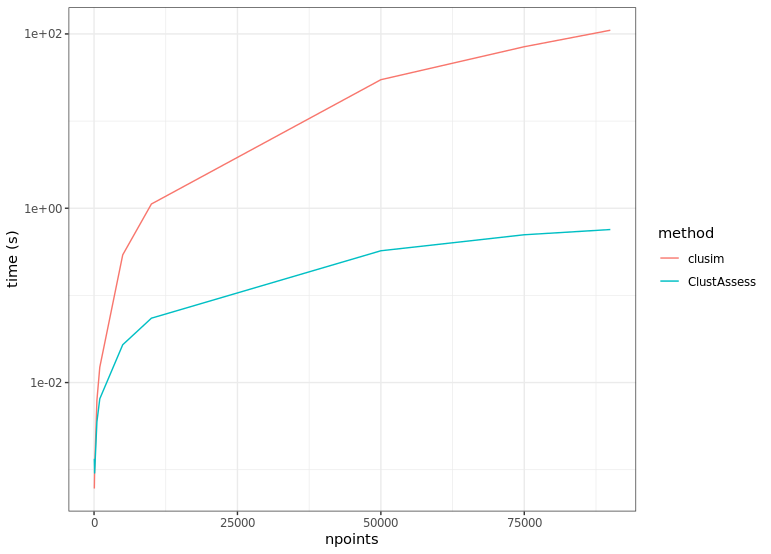
\includegraphics[width=0.7\linewidth]{images/ch4/4_clusim_ca_time.png}
    }
    \caption{\label{fig:comp-time}Clustering distribution with default parameters for Monocle (left) and Seurat (right). The title indicates the default random seed that is used.}
\end{figure}


\begin{table}[]

\resizebox{\textwidth}{!}{
\begin{tabular}{|l||l|l|l|l|l|l|l|l|l|}
\hline
                     & \textbf{50} & \textbf{100} & \textbf{500} & \textbf{1000} & \textbf{5 000} & \textbf{10 000} & \textbf{50 000} & \textbf{75 000} & \textbf{90 000} \\ \hline \hline
\textbf{ClustAssess} & 0.001335    & 0.000918     & 0.003551     & 0.006514      & 0.027171       & 0.054795        & 0.325342        & 0.496565        & 0.57            \\ \hline
\textbf{clusim}      & 0.000608    & 0.000995     & 0.006256     & 0.015005      & 0.291919       & 1.119508        & 29.86761        & 71.3589         & 110.3293        \\ \hline
\end{tabular}}
\caption{\label{tab:comp-time} Time in seconds}
\end{table}

\subsection{Memory consumption comparison}
For analyzing the memory consmuption, we will proceed in a similar manner. We will use the \verb|memory_profiler| module \footnote{Official GitHub repository: \url{https://github.com/pythonprofilers/memory_profiler}} for \verb|clusim|, and the \verb|profvis| package \footnote{Official GitHub repository: \url{https://github.com/rstudio/profvis}} for \verb|ClustAssess|. At each run, we will extract the maximum memory allocation that has occured during the execution.

Figure \ref{fig:comp-mem} illustrates the allocated memory (measure in GiB) during the execution of the task. It is noticeable that \verb|ClustAssess| is memory efficient and requires only a few MiB of memory. On the other side, \verb|clusim| shows the disadvantages of storing the whole affinity matrix into memory: already for 10 000 points the 1 GiB threshold is surpassed (see \ref{tab:comp-mem}) and as the dataset increases, the memory usage also increases exponentially, up to a value of 241 GiB of memory to calculate the ECS of two partitions with 90 000 points.
We note that, at the time of writing, the machines used in daily tasks have between 8 and 32 GB of memory \footnote{Various sources such as \href{https://www.crucial.com/articles/about-memory/how-much-ram-does-my-computer-need}{Crucial} - a memory stick fabricator - indicate that the average user needs between 8 and 16 GB of RAM.}. Therefore, the \verb|clusim| package doesn't scale on big datasets and cannot be used by the casual user.

\begin{figure}[H]
    \centering
    \makebox[\textwidth][c]{
        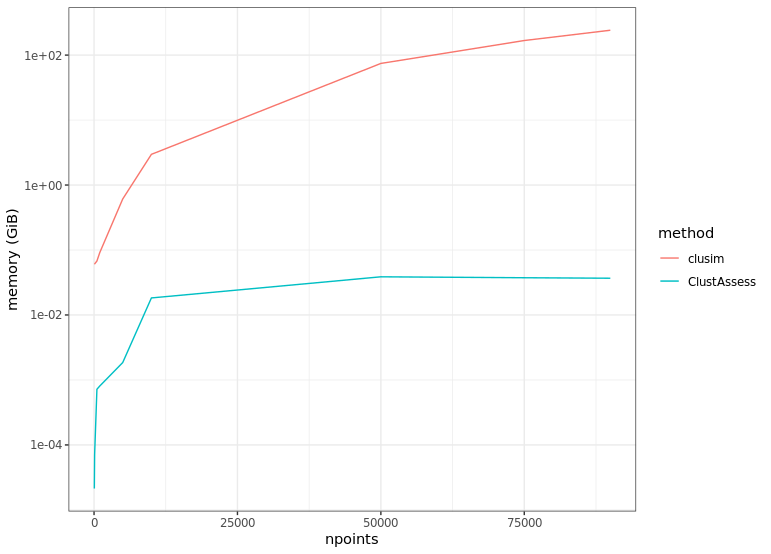
\includegraphics[width=0.7\linewidth]{images/ch4/4_clusim_ca_memory.png}
    }
    \caption{\label{fig:comp-mem}Clustering distribution with default parameters for Monocle (left) and Seurat (right). The title indicates the default random seed that is used.}
\end{figure}


\begin{table}[]

\resizebox{\textwidth}{!}{
\begin{tabular}{|l||l|l|l|l|l|l|l|l|l|}
\hline
                     & \textbf{50} & \textbf{100} & \textbf{500} & \textbf{1000} & \textbf{5 000} & \textbf{10 000} & \textbf{50 000} & \textbf{75 000} & \textbf{90 000} \\ \hline \hline
\textbf{ClustAssess} & 0.000021 & 0.000071 & 0.000719 & 0.000808 & 0.001855 & 0.018308 & 0.038693 & 0.037435 & 0.036799 \\ \hline
\textbf{clusim}      & 0.060688 & 0.061069 & 0.06767 & 0.091365 & 0.610633 & 2.970745 & 74.46173 & 167.6854 & 241.5057 \\ \hline
\end{tabular}}
\caption{\label{tab:comp-mem} Memory in GiB}
\end{table}

\subsection{The impact of the number of clusters}
\verb|ClustAssess| seem to have an efficient way of calculating the Element-Centric Similarity score by using small amounts of memory, but the question is whether its approach scales well on a larger number of clusters. To benchmark its behaviour, we will use the dataset with 90 000 points and vary the number of clusters as described in the previous section.

Figure \ref{fig:comp-k} shows a behaviour that was expected for \verb|ClustAssess|: increasing the number of clusters leads to more unique values to be calculated, hence more execution time required (see the left panel). As for the memory consumption (the right panel), we notice a slight increase that still remains under the threshold of 100 MiB.

Contrary to the expectations, \verb|clusim| seems to perform better when the number of clusters is increased (from 122 seconds for $k = 5$ to 77 for $k = 1000$). Even with this improvement, it still performs worse than \verb|ClustAssess|, which takes 50 seconds to calculate the ECS for $k = 1000$.

\begin{figure}[H]
    \centering
    \makebox[\textwidth][c]{
        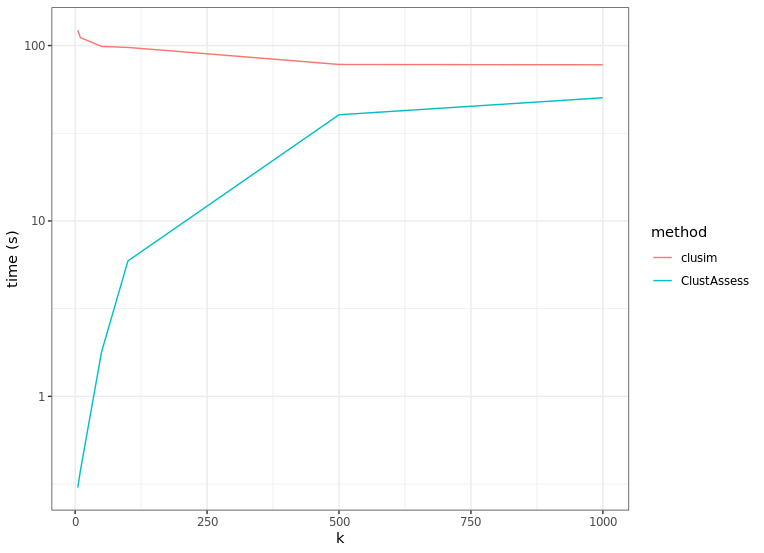
\includegraphics[width=0.5\linewidth]{images/ch4/4_clusim_ca_time_k.png}
        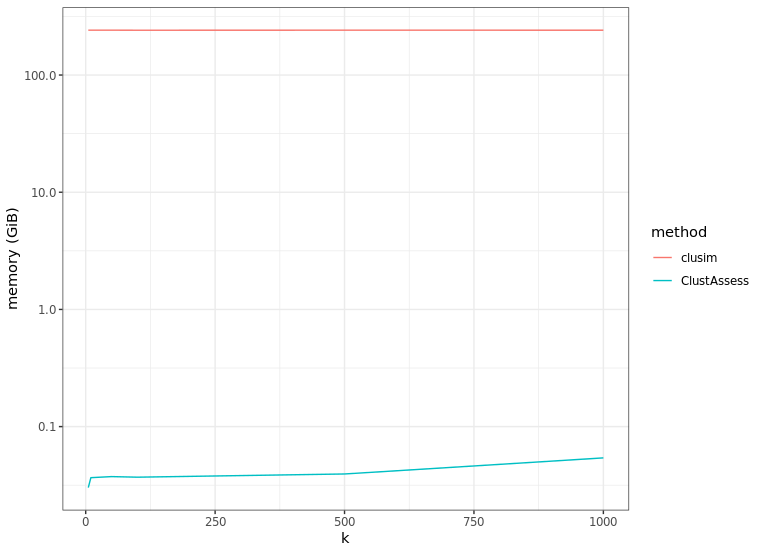
\includegraphics[width=0.5\linewidth]{images/ch4/4_clusim_ca_memory_k.png}
    }
    \caption{\label{fig:comp-k}Clustering distribution with default parameters for Monocle (left) and Seurat (right). The title indicates the default random seed that is used.}
\end{figure}

\subsection{Results accuracy}
The final task is to compare the ECS scores obtained by both packages. Calculating the median of the absolute difference results in an average difference of $5.20417e-17$, which is a negligible difference closer to the machine precision. This leads to the conclusion that the optimization did not affect the accuracy of the ECS results.

\subsection{On the scalability of ClustAssess}
Given the results presented above and the accuracy of the results, the optimized version presented in \verb|ClustAssess| for calculating the ECS score should be considered a more suitable choice, as it is more efficient (especially for a reasonable number of clusters) and it scales linearly as the dataset increases. Also, the low memory consumption is another strong point that highlights the advantages of using our package.

\section{Stability pipeline performance}
Given that for the stability pipeline multiple requires multiple runs of the clustering, an assessment of its scalability and efficiency is required. This section will contain only the analysis of the time execution. Given the memory consumption results from the previous section, we chose not to include additional memory benchmark, as ECS proved to scale well regarding the required space.

Informations regarding the time of executing the whole stability pipeline can also be found at the end of the \href{https://core-bioinformatics.github.io/ClustAssess/articles/stability-based-parameter-assessment.html}{vignette} of the \verb|ClustAssess| package.

\subsection{Benchmark dataset}
The pipeline will be applied on the Mende dataset \cite{Mende2022} which contains a total number of 13 099 cells. The dataset will be subsampled to the following sizes: 1319, 3297, 4396, 6594 and 13099. 

The number of different seeds (or of the runs) will be 30.

\subsection{Benchmark guidelines}
The plots presented in the third chapter are based on object that are created inside the stability pipeline and which contain fields related to the list of partitions, their frequency, the ECC. There are five independent functions that create objects inside the stability pipeline:
\begin{itemize}
    \item \verb|feature_stability|: the object is used for all plots for the Dimensionality reduction step;
    \item \verb|nn_n_conn_comps|: the object is used to create the Connected components target plot from the Graph construction step;
    \item \verb|nn_importance|: the object is used to create the other plots from the same step;
    \item \verb|clustering_importance|: the object is used to create the first two plots related to choosing the community detection algorithm from the Clustering step;
    \item \verb|resolution_importance|: the object is used to create the last two type of plots from the same step.
\end{itemize}

All functions (with the exception of \verb|nn_n_conn_comps|) require the merging of partitions in order to speed up the calculation of the ECC score and to enable the identification of the most frequent partition. Thus, an additional parameter will be the ECS threshold (see Section \ref{sec:part-merge}).

Also, in Section \ref{sec:paral} we mentioned that \verb|ClustAssess| offers support for parallelization. Therefore, the following benchmark will try to evaluate the performance of the five functions with different values for the ECS threshold and the number of cores.

\subsection{Benchmark results}
The results, visually presented in Figure \ref{fig:pipeline-benchmark}, lead to multiple conclusions. First, \\ \verb|nn_n_conn_comps| not only is running fast, but also scales very good as the dataset size increases. The plots are in logarithmic scale, thus looking at panel B, the last row, we can draw the conclusion that the behaviour of this function is sublinear. We can also remark that increasing the number of parallel processes brings significant improvements to the runtime.

The \verb|feature_stability|, \verb|nn_importance| and \verb|clustering_importance| present a similar behaviour, as the panel A of the same figure suggests. One reason might be that the first two contain repeated calls to the dimensional reduction methods, which are computationally expensive. Also, compared to the \verb|nn_n_conn_comps| method, a graph clustering algorithm is applied instead of a method that identifies the connected components. The similar behaviour for the function \verb|clustering_importance| might be explained by the fact that it performs multiple clustering algorithm in a single iteration. Also, SLM usually requires significantly more time to run than the other methods.

The \verb|resolution_importance| function performs better, as it doesn't require any call to a dimensional reduction method and it uses a single clustering algorithm. One thing that is common to the four methods is how they behave when increasing the number of cores. Until a certain point, using multiple processes has a significant gain to the overall execution of the pipeline. However, there is the risk of creating an overhead by adding too many cores. The behaviour is easily noticed in the second Panel for the smallest dataset (red colour): the performance is worsened because the back and forth transfer between the main process and the newly created R instances require more time than the execution of the instances themselves. This happens more frequently when the data is small enough for a run to be executed pretty fast. In the panel B we can observe that if the number of points is increased, the number of situation of performance drops caused by overheads decreases.

As for the ECS threhsold, lowering the threshold to obtain less partitions doesn't seem to help in improving the performance. The reason behind this is that the process of identification of similar partitions that could be merged currently requires the running of pairwise ECS calculation, so the comparison saved after merged are used to obtain the merging.


\begin{figure}[H]
    \centering
    \makebox[\textwidth][c]{
        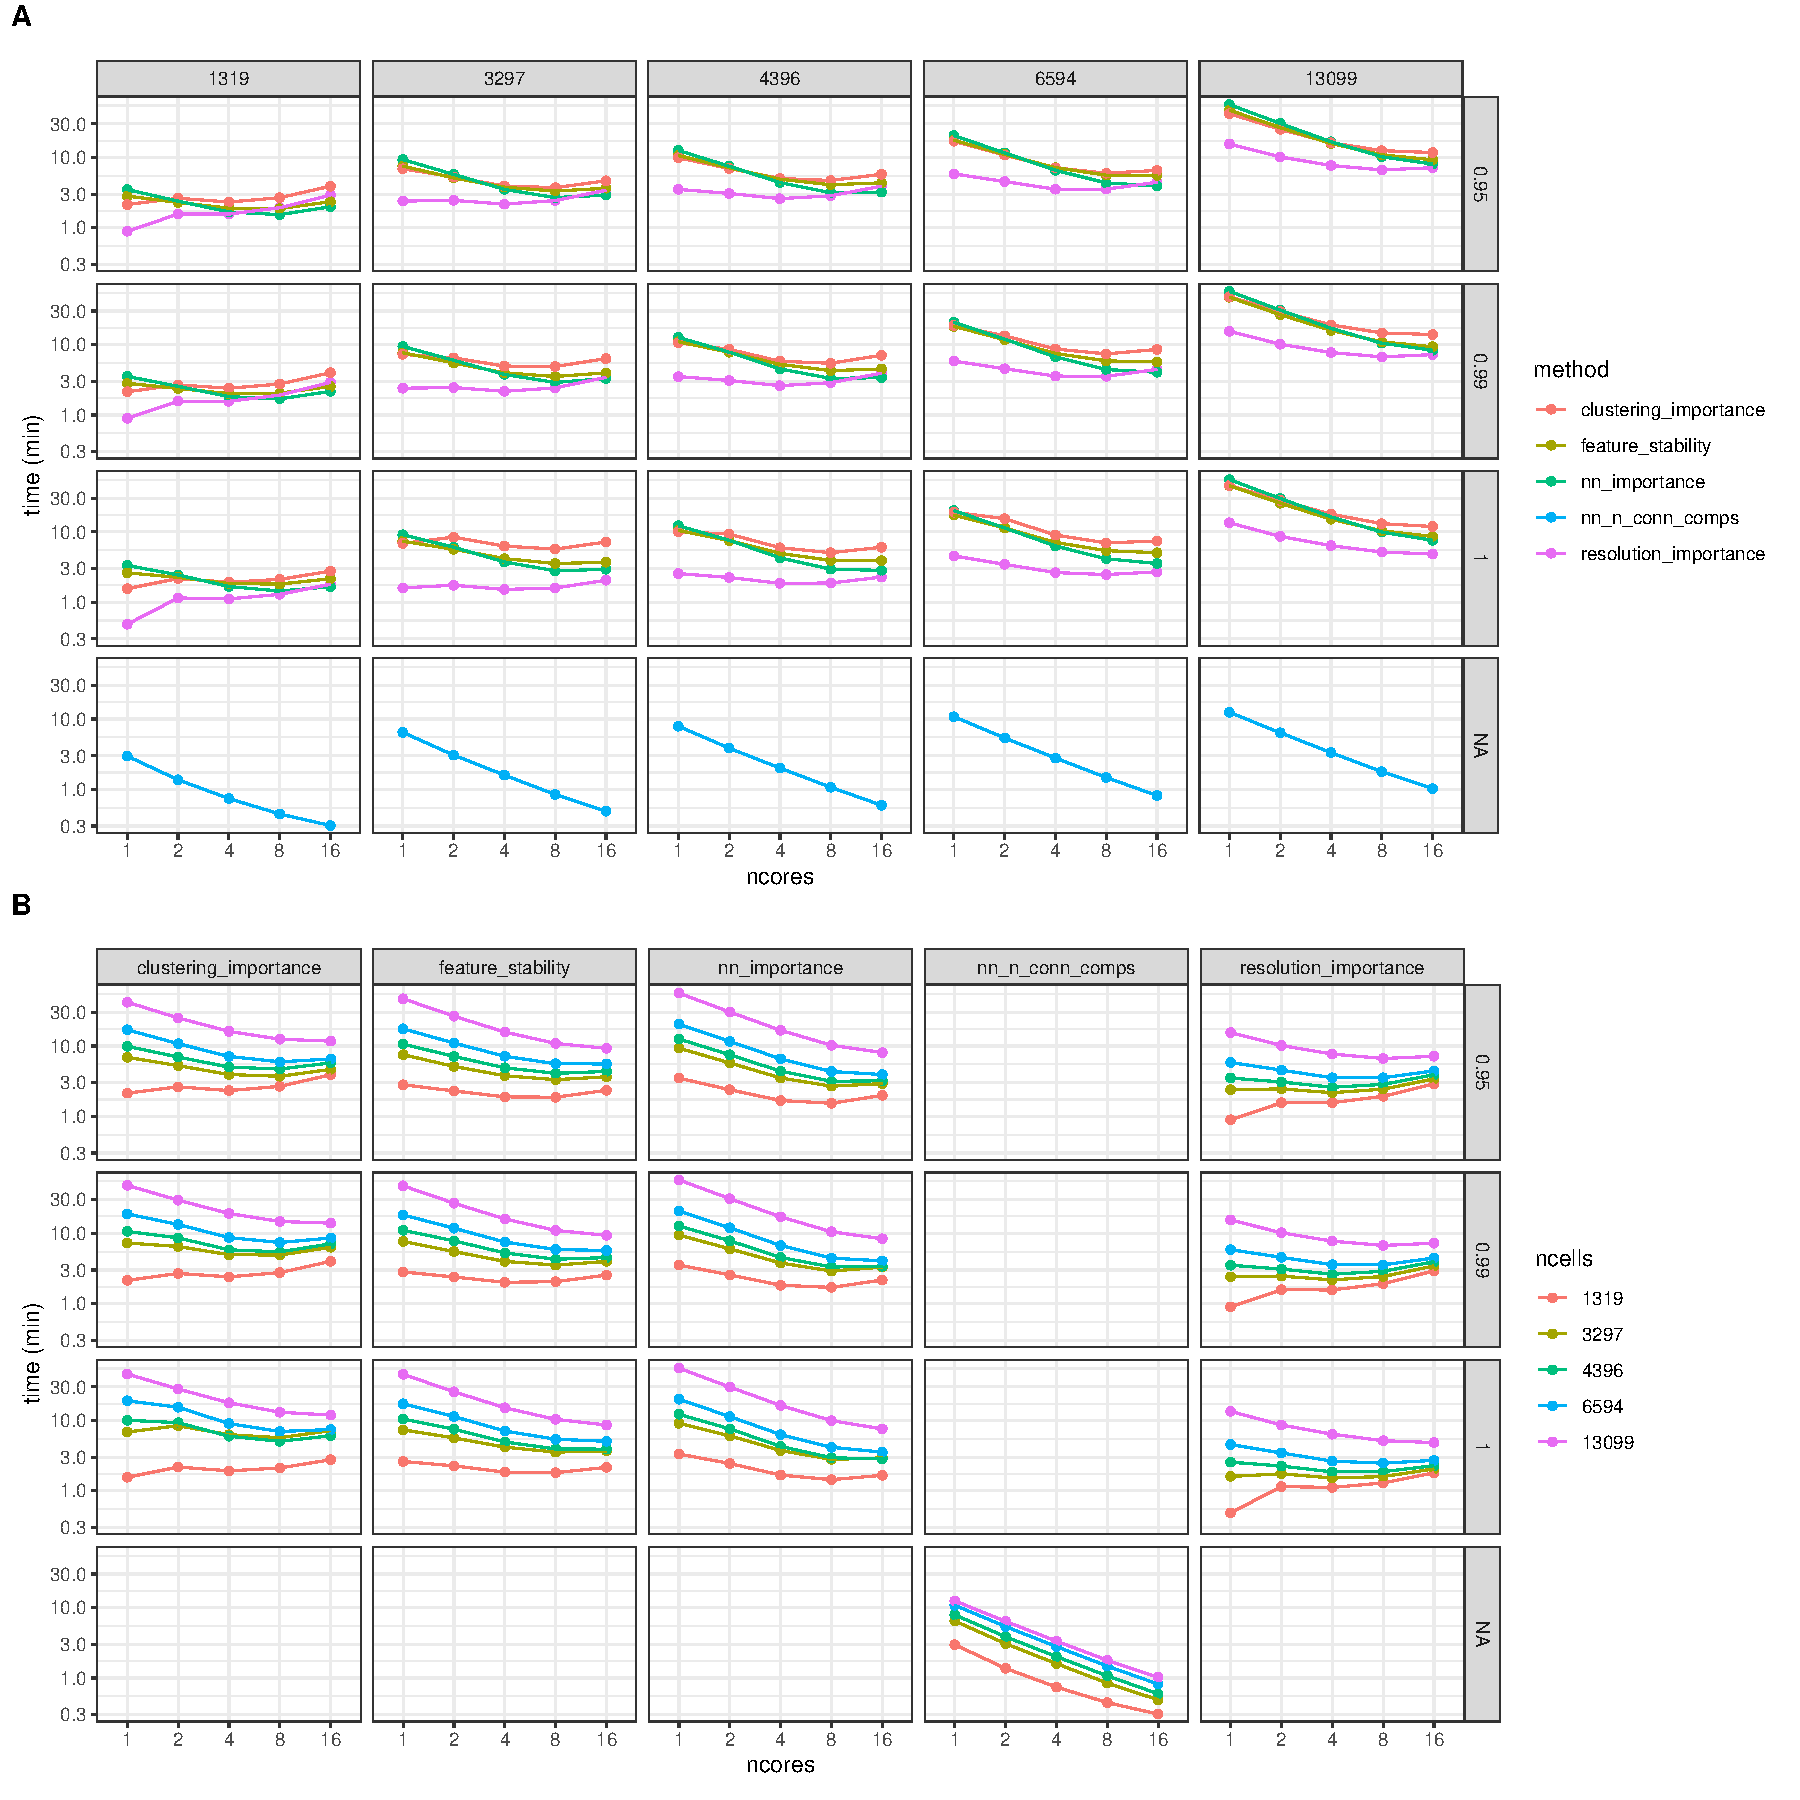
\includegraphics[width=\linewidth]{images/ch4/4_pipeline_benchmark.pdf}
    }
    \caption{\label{fig:pipeline-benchmark}\textbf{Time benchmarks for individual steps of the ClustAssess data-driven evaluation of parameters with respect to the number of cells, ECS thresholds, and number of cores.}
A. Assessment of runtime for an incremental number of cells (columns, corresponding to 10\%, 25\%, 33\%, 50\%, 100\% of the full dataset), subsampled using geometric sketching. The agreement-threshold is controlled via the ECS threshold (rows, the NA row corresponds to the \texttt{nn\_n\_conn\_comps}, as no clustering is performed). On the x-axis we represent the number of cores; the y-axis summarises the runtime (seconds). The colours indicate the methods used to evaluate some parameters of the graph-based clustering pipeline: \texttt{feature\_stability} (the importance of the feature set used as input for the dimensionality reduction), \texttt{nn\_importance} and \texttt{nn\_n\_conn\_comps} (the importance of the base embedding, the number of neighbours and the graph type, graph construction step), \texttt{clustering\_importance} and \texttt{resolution\_importance} (the effect of the clustering method and resolution parameter, community detection step). 
B. Assessment of runtime presented from the perspective of individual methods. We note that the 
%resolution step is minimally affected by the number of cells, whereas the 
runtime increases with more cells; moreover the parallelisation substantially speeds up the processing. Changes in the ECS threshold do not have an impact on runtime.}

\end{figure}

\subsection{Interpreting the results}
The conclusion is that the stability pipeline has scaling capabilites and can be run in a reasonable amount of time for medium-sized datasets. The performance differ from dataset to dataset and could be affected by factors such as:
\begin{itemize}
    \item the clustering algorithm that is used: Louvain and Louvain refined are generally faster than Leiden and SLM (at least in the Seurat's implementation);
    \item the size of the dataset: to obtain the stability plots in a reasonable amount of time, we advise performing a subsampling before running the pipeline;
    \item the number of cores: although it is expected that increasing the number of cores would benefit the performance, there are situations when it could worsen the runtime because of the overheads. A recommendation would be using a number of cores that would lead to a reasonable split of all the runs (if there is a total of 32 runs and we set the number of cores to 16, there is a high chance of reaching the overhead). Also, for smaller datasets each run is executed faster, therefore the overhead threshold will vary depending on the size of the provided data.
\end{itemize}
    
    \chapter*{Conclusions and Future Work} 
\addcontentsline{toc}{chapter}{Conclusions and Future Work}

Clustering comparison metrics are important for benchmarking and evaluating the output of a clustering method when a ground truth is provided. These scores can also be used to compare different clustering methods or different configurations i.e. different values for the parameters of the same algorithm. Element-Centric Similarity (ECS) is a score that is not biased on the size, shape or the number of clusters and which provides information about the global and local agreement between two partitions. The \verb|ClustAssess| package provides the first R implementation of this score which also performs the calculation in an scalable, both space and time optimized manner.

We also emphasized the importance of the parameter configuration on the clustering output, but also the undesired impact that factors such as random seed can have on the final results. The solution we proposed in \verb|ClustAssess| was to provide a stability pipeline, which follows the steps from the PhenoGraph algorithm. The purpose of the pipeline is to provide visual assessments of the stability and robustness of different configuration at the change of random seed and to assist the user into choosing a configuration that leads to consistent, not seed reliant results.

As future work we are looking to furtherly optimize the calculation of the ECS score based on the final form as it was presented in Remark \ref{remark:ecs-constant}. At the moment only the case of disjoint partitions was optimized, so the calculation of the ECS score between overlapping or hierarhical partitions is also something to be improved. 

The introduction of the ECS threshold term and of the evaluation of close similarity between partitions could lead to further improvements in the time execution. The issue is that a specific value of the ECS value changes its interpretation when the size of the datasets changes. A ECS value of 0.99 could be interpreted as only a few points labeled differently for small datasets or entire region differences for larger ones. We intend in finding a correspondence between the ECS value and the possible number of points that changed their cluster label.

Finally, we are constantly planning on improving the quality and the usefulness of the plots involved in the stability pipeline.

    \newpage

    Title: ClustAssess: Tools for Assessing Clustering

    Student name: Munteanu Andi
    
    Coordinator: Conf dr. Liviu Ciortuz \\

    The thesis is based on the ClustAssess paper \cite{clustassess}, where I contributed as an author and developer of the R package. \\

    
    Clustering is an unsupervised method that is used to classify and label points based on different similarity metrics. Comparing to the supervised classifiers, clustering algorithms do not require training and using a model and are most suitable when the label of the points are not priorly known and are inferred based on the features that describe them.

    Depending on the approach, clustering methods can be divided in multiple categories, such as centroid-based (k-means), density-based (DBSCAN), hierarchical, distribution-based (EM). One approach that gained popularity in the last decades are the graph-based clustering. Some of its advantages is providing flexibility when it comes to the cluster shapes and sizes, or the scalability.

    Our thesis focus is set on the community detection techniques, that is graph-based clustering approach that rely on optimizing an objective function (also known in literature as quality function or quality metric, as it tries to evaluate the quality of the clustering by encouraging high density of edges inside clusters and as few intrer-cluster links as possible). This method is intensively used, as it manages to obtain close to optimal results in an efficient time. 

    Given that many datasets are provided as points displayed on a high-dimensional space, a methodology that enables the use of community detection method on this data is required. Our reference is the PhenoGraph algorithm presented by Levine et. al \cite{Levine2015}, that establishes a pipeline that firstly applies a dimensionality reduction technique (a linear one such as PCA or non-linear one such as UMAP), then generates a graph using the Nearest Neighbour algorithm. The resulting graph is then used as input for the community detection algorithm.

    The PhenoGraph pipeline has been used frequently in several domains. One of them is the downstream analysis of biological data, where the goal is to cluster the cells in multiple groups that will be used to infer some biological conclusions. The input data is usually provided as a matrix that has cells sampled from different donors at different timepoints on the rows. The columns represent the genes that can be expressed in the cells. Given that the human genome contains approximately 30.000 genes, the input space is a high dimensional one, which makes the PhenoGraph pipeline a suitable choice for processing the data. Also, using graphs to represent data is a more appropiate way to describe the cell-cell interaction.

    The current state-of the art of processing the biological data is thus using the PhenoGraph pipeline: for dimensionality reduction, approximate PCA using the Lanczos bidiagonalization method \cite{Baglama2016IRLBAFP} or UMAP \cite{mcinnes2018uniform}; for graph building, the Nearest Neighbour algorithm \cite{Xu2015}; for community detection, Louvain \cite{Blondel2008b}, Louvain with multilevel refinement \cite{Rotta2011}, Smart Local Moving Algorithm \cite{Waltman2013} and Leiden \cite{Traag2019a}. 

    Currently, some of the most popular tools used for analyzing single-cell data are Seurat \cite{Hao2021}, Monocle \cite{Cao2019} and SCANPY \cite{Wolf2018}. Our thesis makes a comparison between Seurat and Monocle regarding the implementation of the PhenoGraph pipeline. This was motivated by the significant differences between the results of the two packages and the subsequent divergent biological interpretation of the obtained partitions. The question we wanted to answer is whether this differences are caused by computational or biological factors (such as sequencing depth or how the data was pre-processed).

    In our thesis we showcase how the divergence was caused by using parameters values that do not match. The conclusion we draw is that tuning the algorithm's parameters is essential in obtaining reproducable results. Given the stochastic nature of the algorithms that are involved in the pipeline, we also noticed how changing the random seed value is a direct factor that affects the clustering output.

    The instability caused by random seed was previously identified in several papers that pursued the algorithm modification in order to achieve stability. Such example is kmeans++ \cite{kmeanspp}, where the authors replaced the random initialization of the centroids with assigning probabilities of selection based on the distance to the existing center points. Another example is provided in the clust-perturb algorithm proposed by Stacey et al. \cite{STACEY2021}, where the robustness is evaluated by introducing random noise in the graph.

    Our work is focused on providing a pipeline that follows the algorithms involved in the PhenoGraph. The package that we developed its purposed to provide informative plots that would give the user insight about how different parameters impact the number of clusters and the partitioning. Another purpose that we try to achieve is to evaluate and provide insight about parameters configuration that are robust to the change of seeds. The robustness is determined by using Element Centric Similarity (ECS) \cite{Gates2019}, a measurement that determines how similar are two clustering of the same data. 




    \bibliographystyle{unsrt}
    \bibliography{chapters/bibliography}{}
    
\end{document}
